\documentclass[11pt,letterpaper,boxed]{pset}

\usepackage[margin=0.75in]{geometry}
\usepackage{ulem}

\begin{document}

    \problemlist{PHYS051 HW01}
    \begin{center}
    	P25.4, E26.10, *E25.16, E26.16, E26.21, P26.7
    \end{center}
    
    \begin{problem} [P25.4]
    	Two similar tiny balls of mass \textit{m} are hung from silk threads of length $L$ and carry equal charges \textit{q} as in Fig. 25-22. Assume that $\theta$ is so small that tan $\theta$ can be replaced by its approximate equal, sin $\theta$.
    	
    	\begin{itemize}
    	    \item [(a)] To this approximation show that, for equilibrium, 
    	    \[ x = (\frac{q^2 L}{2 \pi \epsilon_0 mg})^{1/3} \]
    	    where \textit{x} is the separation between the balls.
    	    \item [(b)] If \textit{L} = 122 cm, \textit{m} = 11.2 g, and \textit{x} = 4.70 cm, what is the value of \textit{q}?
    	\end{itemize}
    \end{problem}
    
    \begin{figure*} [ht]
        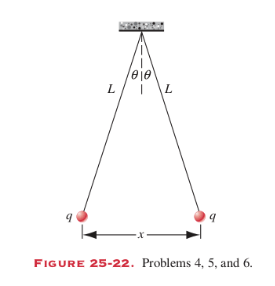
\includegraphics[width=175px]{HW1Images/P25-4.png}
        \label{fig:P25-4}
    \end{figure*}
    \newpage
    
    \begin{problem} [E26.10]
    	In Fig. 26-5, assume that both charges are positive. Show that the magnitude of \textit{E} at point \textit{P} in that figure, assuming $x \gg d$, is given by
    	
    	\[ E = \frac{1}{4\pi\epsilon_0}\frac{2q}{x^2} \]
    	
    	Please comment on how and why your answer differs from the dipole result.
    \end{problem}
    
    \begin{figure*} [ht]
        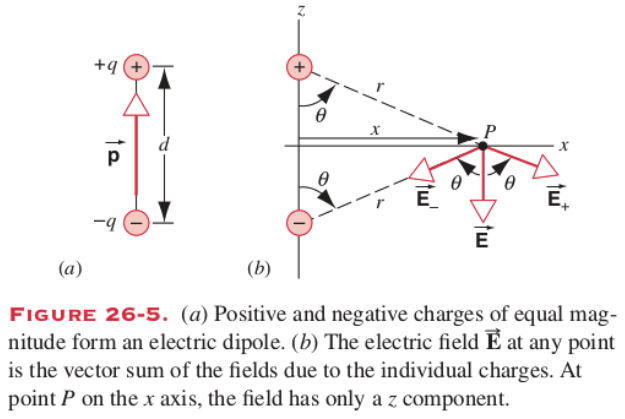
\includegraphics[width=250px]{HW1Images/E26-10.png}
        \label{fig:E26-10}
    \end{figure*}
    \newpage
    
    \begin{problem} [*E25.16]
    	Find the force on a positive point charge \textit{q} located a distance of \textit{x} from the end of a rod of length \textit{L} with uniformly distributed positive charge \textit{Q}. (See Fig. 25-21).
    \end{problem}
    
    \begin{figure*} [ht]
        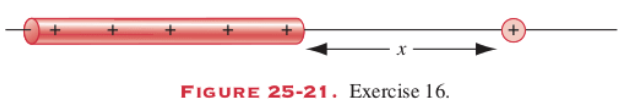
\includegraphics[width=250px]{HW1Images/E25-16.png}
        \label{fig:E25-16}
    \end{figure*}
    \newpage
    
    \begin{problem} [E26.16]
    	A thin glass rod is bent into a semicircle of radius \textit{r}. A charge $+q$ is uniformly distributed along the upper half and a charge of $-q$ is uniformly distributed along the lower half, as shown in Fig. 26-28. Find the electric field \textbf{$\Vec{E}$} at $P$, the center of the semicircle.
    \end{problem}
    
    \begin{figure*} [ht]
        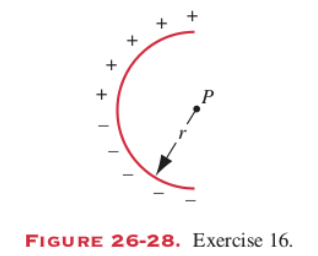
\includegraphics[width=150px]{HW1Images/E26-16.png}
        \label{fig:E26-16}
    \end{figure*}
    \newpage
    
    \begin{problem} [E26.21]
    	Sketch qualitatively the field lines associated with a thin, circular, uniformly charged disk of radius $R$. (Hint: Consider as limiting cases points very close to the disk, where the electric field is perpendicular to the surface, and points very far from it, where the electric field is like that of a point charge.)
    \end{problem}
    \newpage
    
    \begin{problem} [P26.7]
    	A thin nonconducting rod of finite length $L$ carries a uniform linear charge density $+\lambda$ on the top half and a uniform charge density $-\lambda$ on the bottom half; compare to Fig. 26-6.
    	
    	\begin{itemize}
    	    \item [(a)] Use a symmetry argument to determine the direction of the electric field at $P$ due to the rod.
    	    \item [(b)] Find \textbf{$\Vec{E}$} at $P$.
    	    \item [(c)] Take the limit of this expression for large $y$. How does it depend on $y$? What does this remind you of?
    	\end{itemize}
    \end{problem}
    
    \begin{figure*} [ht]
        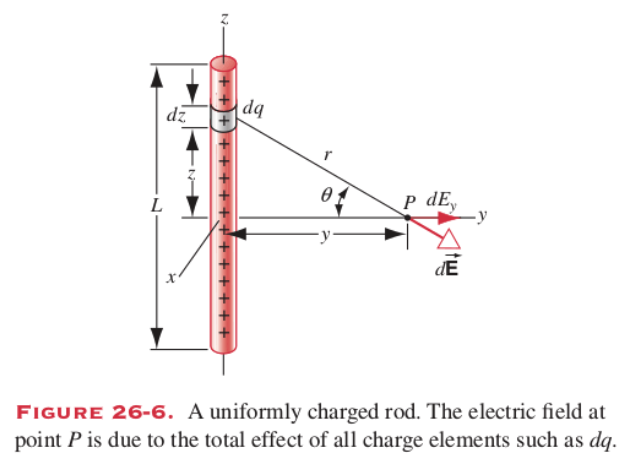
\includegraphics[width=225px]{HW1Images/P26-7.png}
        \label{fig:P26-7}
    \end{figure*}
    
    \newpage
\end{document}